\documentclass[submit]{../harvardml}

\course{CS1810-S25}
\assignment{Assignment \#3}
\duedate{11:59pm EST, March 14th, 2025}

\usepackage{../common}
\usepackage[OT1]{fontenc}
\usepackage[colorlinks,citecolor=blue,urlcolor=blue]{hyperref}
\usepackage{graphicx}
\usepackage{amsmath}
\usepackage{amssymb}
\usepackage{framed}
\usepackage{color}
\usepackage{listings}
\usepackage{enumitem}
\usepackage{comment}

%%%%%%%%%%%%%%%%%%%%%%%%%%%%%%%%%%%%%%%%%%%
%% Solution environment
\usepackage{xcolor}
\newenvironment{solution}{
    \vspace{2mm}
    \color{blue}\noindent\textbf{Solution}:
}{}
%%%%%%%%%%%%%%%%%%%%%%%%%%%%%%%%%%%%%%%%%%%

% \excludecomment{solution} % UNCOMMENT TO HIDE SOLUTIONS

% Student answer environment (used for answer templates)
\newenvironment{answer}
  {\section*{Solution}}
{}

\DeclareMathOperator*{\mean}{\mathbb{E}}

\lstset{
  language=Python,
  basicstyle=\ttfamily,
  keywordstyle=\color{blue}\bfseries,
  commentstyle=\color{red},
  stringstyle=\color{green},
  frame=single,
  showstringspaces=false,
}

\definecolor{verbgray}{gray}{0.9}

\lstnewenvironment{csv}{%
  \lstset{backgroundcolor=\color{verbgray},
  frame=single,
  framerule=0pt,
  basicstyle=\ttfamily,
  columns=fullflexible}}{}

\begin{document}

\begin{center}
  {\Large Homework 3: Bayesian Methods and Neural Networks}\\
\end{center}

\subsection*{Introduction}

This homework is about Bayesian methods and neural networks.

\begin{enumerate}
  \item You'll explore the Bayesian paradigm and compare it with the frequentist paradigm for the Beta-Binomial conjugate pair.
  \item You'll derive the backpropagation algorithm for a single-hidden-layer neural network for the binary classification task.
  \item You'll write some code using the PyTorch library for an image classification task.
  \item You'll consider the opportunities and limitations of ML applications and learn to anticipate possible exploits of these systems.
\end{enumerate}

As always, please start early and come to office hours with questions!

\subsection*{Resources and Submission Instructions}
You may want to consider the lecture notes from Feb 18th to 27th (weeks 4 and 5).

Please type your solutions after the corresponding problems using this
\LaTeX\ template, and start each problem on a new page.

Please submit the \textbf{writeup PDF to the Gradescope assignment `HW3'}. Remember to assign pages for each question.  \textbf{You must include your plots in your writeup PDF. } The supplemental files will only be checked in special cases, e.g. honor code issues, etc.

Please submit your \textbf{\LaTeX\ file and code files to the Gradescope assignment `HW3 - Supplemental'}. \\


\newpage

%%%%%%%%%%%%%%%%%%%%%%%%%%%%%%%%%%%%%%%%%%%%%
% Problem 1
%%%%%%%%%%%%%%%%%%%%%%%%%%%%%%%%%%%%%%%%%%%%%

\begin{problem}[Connecting Bayesian and Frequentist Approaches, 40 pts]

In this question, we will gain practice with Bayesian modeling and
compare it with the frequentist paradigm.
In class, we discussed \emph{Normal-Normal conjugacy.} Now
we will turn to \emph{Beta-Binomial conjugacy.} This model can be
visualized in the following way.
You observe a fixed number \(N\) of coin flips (either
heads or tails) of which \(Y\) (a random variable) are heads. You assume that these are
drawn by flipping a coin with an unknown probability \(\theta\) of
landing heads. That is, we choose a \textbf{Binomial likelihood}
\(Y \sim \mathrm{Bin}(N, \theta)\). The PMF of this distribution is
given by

\[
  p(Y=y) = {N \choose y} \theta^{y} (1-\theta)^{N-y}.
\]

\begin{enumerate}
  \item[1.]
    \textbf{Frequentist paradigm and MLE.} The (log) likelihood is all we
    need for frequentist inference. Derive the MLE estimate for \(\theta\)
    given the observations \(Y = y\). That is, find
    \[\arg \max_{\theta} \log p(Y = y \mid \theta).\]

  \item[2.]
    \textbf{Beta-Binomial conjugacy.} Under the Bayesian paradigm, we must specify a
    prior distribution for the unknown parameter \(\theta\). We choose a \textbf{Beta prior}
    \(\theta \sim \mathrm{Beta}(\alpha, \beta)\). The PDF of this
    distribution is given by

    \[
      p(\theta) \propto \theta^{\alpha - 1} (1-\theta)^{\beta - 1}.
    \]

    When the prior and posterior belong to the same distribution family, we
    call the prior-and-likelihood pair a \textbf{conjugate pair.}

    For the rest of the problem, feel free to cite that the mean of the \(\mathrm{Beta}(\alpha, \beta)\) distribution is
    \[\mean[\theta] = \frac{\alpha}{\alpha+\beta},\]
    the mode is
    \[\arg\max_\theta p(\theta) = \frac{\alpha-1}{\alpha+\beta-2},\]
    and the variance is
    \[
      \mathrm{Var}(\theta) = \frac{\alpha \beta}{(\alpha + \beta)^2 (\alpha + \beta + 1)}.
    \]

    \begin{enumerate}
      \item
            Qualitatively speaking, what does the $\mathrm{Beta}(\alpha, \beta)$ distribution look like for different $\alpha$ and $\beta$? You can either plot this yourself or see \href{https://en.wikipedia.org/wiki/Beta_distribution}{its Wikipedia page}. What distribution does $\mathrm{Beta}(1, 1)$ correspond to?

      \item
            Show that the posterior
            \(p(\theta \mid Y=y)\) is indeed Beta and derive its parameters. This proves that a Beta prior and a Binomial likelihood form a conjugate pair; in other words, the Beta distribution is a \textbf{conjugate prior} for the Binomial distribution.

            \textbf{Hint} (for convenience in calculation): Do you need to calculate the normalizing constant?
    \end{enumerate}
\end{enumerate}
\end{problem}

\newpage

\begin{framed}
  \begin{enumerate}
    \item[3.]
      \textbf{Posterior mean and mode.} Often we wish to work with just a
      single point estimate of the posterior. Two commonly used point
      estimates are the \emph{posterior mean} and the \emph{posterior mode}
      (a.k.a. the maximum a posteriori (MAP) estimate).

      \begin{enumerate}
        \item
              Discuss the advantages and disadvantages of using posterior point
              estimates. Which of these are relevant for our Beta-Binomial conjugate pair?

        \item
              Using your results from part 2, write down

              \begin{enumerate}
                \item the posterior mean estimate \(\theta_{\text{post mean}} = \mean [\theta \mid Y = y]\),
                \item the posterior MAP estimate \(\theta_{\text{MAP}}=\arg \max_{\theta}p(\theta \mid Y=y)\),
                \item and the posterior variance $\mathrm{Var}(\theta \mid Y = y) = \mean[\theta^2 \mid Y = y] - (\mean[\theta \mid Y = y])^2$.
              \end{enumerate}

              \textbf{Hint}: Do you need to rederive anything? (This exercise should illustrate the power of conjugate priors!)

      \end{enumerate}

    \item[4.]
      \textbf{Prior-posterior connections.}

      \begin{enumerate}
        \item
              Explain in your own words how \(\alpha\) and \(\beta\) affect the
              MAP estimate. How would you set \(\alpha\) and \(\beta\) to reflect
              a prior belief that the coin is fair (i.e.~shows heads and tails
              with equal probability)? (Be careful that your answer does \emph{not} give high probability to an ``always heads'' coin or ``always tails'' coin!)

        \item Now let's analyze the variances of our prior and posterior distributions. Consider the case when $\alpha = \beta$. (If you'd enjoy it, consider the general case for better understanding.) Please write at most two sentences per point.
              \begin{enumerate}
                \item How does the variance of the prior relate to the variance of the posterior?
                \item How might you use the prior variance to encode a stronger or weaker prior belief?
                \item How does the posterior variance change as we observe more samples $n$?
              \end{enumerate}
      \end{enumerate}

    \item[5.]
      \textbf{Analysis and connection to frequentism.}

      \begin{enumerate}
        \item
              Write a loss function \(\ell(\theta) \in \mathbb{R}\) in terms of
              \(\theta, y, n, \alpha, \beta\) such that minimizing \(\ell\) is
              equivalent to calculating the MAP estimate,
              i.e.~\(\theta_{\text{MAP}} = \arg \min_{\theta} \ell(\theta)\). Your
              function should be a sum of:
              \begin{enumerate}
                \item a mean-squared-error term (which should loosely resemble $(y - \hat y)^2$)
                \item a
                      regularization term \(g(\theta) = - a \theta + b \theta^{2}\) for some $a, b$.
              \end{enumerate}

              Can you interpret the regularization term?

              \textbf{Hint}: Work backwards from part 1 to derive the MSE term and from the MAP in part 2 to get the regularization term. Watch out for the signs! For the interpretation, complete the square and then compare your expression with the prior mode in part 2.
        \item
              What happens to both $\theta_{\text{post mean}}$ and $\theta_{\text{MAP}}$ as \(n \to \infty\)? Compare this to the MLE estimate.
              (Remember to account for the change in \(y\).)
      \end{enumerate}

  \end{enumerate}

\end{framed}

\begin{answer}
  \begin{enumerate}
    \item[1.]
      \textbf{MLE Derivation:}\\
      The log-likelihood for the Binomial distribution is given by
      \[
      \ell(\theta) = \log p(Y=y \mid \theta) = \log \binom{N}{y} + y\log\theta + (N-y)\log(1-\theta).
      \]
      Since \(\binom{N}{y}\) does not depend on \(\theta\), we maximize
      \[
      \tilde{\ell}(\theta) = y\log\theta + (N-y)\log(1-\theta).
      \]
      Differentiating with respect to \(\theta\) and setting the derivative to zero:
      \[
      \frac{d\tilde{\ell}}{d\theta} = \frac{y}{\theta} - \frac{N-y}{1-\theta} = 0.
      \]
      Solving for \(\theta\):
      \[
      \frac{y}{\theta} = \frac{N-y}{1-\theta} \quad \Rightarrow \quad y(1-\theta) = (N-y)\theta,
      \]
      \[
      y = N\theta \quad \Rightarrow \quad \hat{\theta}_{\text{MLE}} = \frac{y}{N}.
      \]

    \item[2.]
      \begin{enumerate}
        \item \textbf{Qualitative Description of the Beta Distribution:}\\[1mm]
              The \(\mathrm{Beta}(\alpha,\beta)\) distribution is defined on the interval \([0,1]\) and its shape depends on the parameters. For example, when \(\alpha>1\) and \(\beta>1\) the distribution is unimodal and bell-shaped; when \(\alpha<1\) and \(\beta<1\) it is U-shaped; and when one parameter is less than 1 and the other greater than 1, the distribution is skewed. In particular, \(\mathrm{Beta}(1,1)\) corresponds to the uniform distribution on \([0,1]\).

        \item \textbf{Posterior Derivation:}\\[1mm]
              Given the prior
              \[
              p(\theta) \propto \theta^{\alpha-1}(1-\theta)^{\beta-1},
              \]
              and the likelihood
              \[
              p(Y=y\mid\theta) \propto \theta^{y}(1-\theta)^{N-y},
              \]
              the unnormalized posterior is
              \[
              p(\theta\mid Y=y) \propto \theta^{y+\alpha-1}(1-\theta)^{N-y+\beta-1}.
              \]
              Recognizing this as the kernel of a Beta distribution, we conclude that
              \[
              \theta\mid Y=y \sim \mathrm{Beta}(\alpha+y,\beta+N-y).
              \]
      \end{enumerate}

    \item[3.]
      \begin{enumerate}
        \item \textbf{Discussion on Posterior Point Estimates:}\\[1mm]
              The posterior mean takes into account the entire distribution, providing an average estimate that minimizes squared error loss, whereas the posterior mode (MAP) gives the most probable value but ignores distributional uncertainty. For the Beta-Binomial conjugate pair, both are easily computed; however, the MAP can be sensitive to the prior when \(\alpha\) or \(\beta\) are small, while the mean offers a smoother summary.
              
        \item \textbf{Posterior Estimates:}\\[1mm]
              \begin{align*}
                \theta_{\text{post mean}} &= \mean[\theta\mid Y=y] = \frac{\alpha+y}{\alpha+\beta+N},\\[1mm]
                \theta_{\text{MAP}} &= \arg\max_{\theta} p(\theta\mid Y=y) = \frac{\alpha+y-1}{\alpha+\beta+N-2},\\[1mm]
                \mathrm{Var}(\theta\mid Y=y) &= \frac{(\alpha+y)(\beta+N-y)}{(\alpha+\beta+N)^2(\alpha+\beta+N+1)}.
              \end{align*}
      \end{enumerate}

    \item[4.]
      \begin{enumerate}
        \item \textbf{Effect of \(\alpha\) and \(\beta\) on the MAP Estimate:}\\[1mm]
              The parameters \(\alpha\) and \(\beta\) act as pseudo-counts that effectively add to the observed data, shifting the MAP estimate toward the prior mode. To encode a belief that the coin is fair, one should choose \(\alpha = \beta\) (with values greater than 1 to avoid degenerate behavior), ensuring that the prior mode is at 0.5.
              
        \item \textbf{Variance Analysis when \(\alpha = \beta\):}\\[1mm]
              \begin{enumerate}
                \item When \(\alpha = \beta\), a small value of \(\alpha\) (i.e., a diffuse prior) leads to a large variance, while a large \(\alpha\) yields a concentrated (low-variance) prior; the posterior variance is always lower than the prior variance due to the information added by the data.
                \item By choosing larger values of \(\alpha\) and \(\beta\), one encodes a stronger prior belief (resulting in a smaller prior variance); conversely, smaller values indicate a weaker belief (larger variance).
                \item As the number of observed samples \(N\) increases, the posterior variance decreases, reflecting increased certainty about \(\theta\).
              \end{enumerate}
      \end{enumerate}

    \item[5.]
      \begin{enumerate}
        \item \textbf{Loss Function Formulation:}\\[1mm]
              The negative log-likelihood (ignoring constant terms) for the Binomial model would be minimized at the MLE, corresponding roughly to a term that looks like
              \[
              \text{MSE term: } M(\theta) = (y-N\theta)^2.
              \]
              To shift this optimum from the MLE \(\theta=\frac{y}{N}\) to the MAP \(\theta=\frac{\alpha+y-1}{\alpha+\beta+N-2}\), we add a regularization term derived from the negative log-prior.
              \[
              R(\theta) = -2N(\alpha-1)\theta + N(\alpha+\beta-2)\theta^2,
              \]
              the overall loss function becomes
              \[
              \ell(\theta) = (y-N\theta)^2 -2N(\alpha-1)\theta + N(\alpha+\beta-2)\theta^2.
              \]
              \textbf{Interpretation:} The regularization term acts as a penalty derived from the prior information, effectively adding pseudo-observations that pull the estimate towards the prior mode.
              
        \item \textbf{Asymptotic Behavior:}\\[1mm]
              As \(N \to \infty\), the influence of the prior (i.e., the terms involving \(\alpha\) and \(\beta\)) diminishes relative to the data. Consequently, both the posterior mean and the MAP estimate converge to the MLE \(\frac{y}{N}\), reflecting that with abundant data the prior becomes negligible.
      \end{enumerate}

  \end{enumerate}
\end{answer}


\newpage

%%%%%%%%%%%%%%%%%%%%%%%%%%%%%%%%%%%%%%%%%%%%%
% Problem 2
%%%%%%%%%%%%%%%%%%%%%%%%%%%%%%%%%%%%%%%%%%%%%

\begin{problem}[Neural Networks, 20 pts]

In this problem, we will take a closer look at how gradients are calculated for backpropagation with a simple multi-layer perceptron (MLP). The MLP will consist of a first fully connected layer with a sigmoid activation, followed by a one-dimensional, second fully connected layer with a sigmoid activation to get a prediction for a binary classification problem. We use non-linear activation functions as the composition of linear functions is linear. Assume bias has not been merged. Let:
\begin{itemize}
  \item $\bold{W}_1$ be the weights of the first layer, $\bold{b}_1$ be the bias of the first layer.
  \item $\bold{W}_2$ be the weights of the second layer, $\bold{b}_2$ be the bias of the second layer.
\end{itemize}

The described architecture can be written mathematically as: $$\hat{y} = \sigma(\bold{W}_2 \left[\sigma \left(\bold{W}_1 \bold{x} + \bold{b}_1\right)\right] + \bold{b}_2)$$

where $\hat{y}$ is a scalar output of the net when passing in the single datapoint $\bold{x}$ (represented as a column vector), the additions are element wise additions, and the sigmoid is an element wise sigmoid.

\begin{enumerate}
  \item Let:
        \begin{itemize}
          \item $N$ be the number of datapoints we have
          \item $M$ be the dimensionality of the data
          \item $H$ be the size of the hidden dimension of the first layer. Here, hidden dimension is used to describe the dimension of the resulting value after going through the layer. Based on the problem description, the hidden dimension of the second layer should be 1.
        \end{itemize}

        Write out the dimensionality of each of the parameters, and of the intermediate variables:

        \begin{align*}
          \bold{a}_1 & = \bold{W}_1 \bold{x} + \bold{b}_1,
                     & \bold{z}_1 = \sigma(\bold{a}_1)       \\
          a_2        & = \bold{W}_2 \bold{z}_1 + \bold{b}_2,
                     & \hat{y} = z_2 = \sigma(a_2)
        \end{align*}

        and make sure they work with the mathematical operations described above. Examining shapes is one of the key ways to debug your code, and can be done using .shape after any numpy array.

  \item  We will derive the gradients for each of the parameters, which can then be used along with gradient descent to find weights that improve our model's performance. For this question, assume there is only one datapoint $\bold{x}$, and that our loss is $L = -(y \log (\hat{y}) + (1 - y) \log (1 - \hat{y}))$. For all questions, the chain rule will be useful.
        \begin{enumerate}
          \item Find $\frac{\partial L}{\partial b_2}$.

          \item Find $\frac{\partial L}{\partial W_2^h}$, where $W_2^h$ represents the $h$th element of $\bold{W}_2$.

          \item Find $\frac{\partial L}{\partial b_1^h}$, where $b_1^h$ represents the $h$th element of $\bold{b}_1$. (\textbf{Hint}: Note that only the $h$th element of $\bold{a}_1$ and $\bold{z}_1$ depend on $b_1^h$ - this should help you with how to use the chain rule.)

          \item Find $\frac{\partial L}{\partial W_1^{h, j}}$, where  $W_1^{h,j}$ represents the element in row $h$, column $j$ in $\bold{W}_1$.

        \end{enumerate}

\end{enumerate}

\end{problem}

\newpage

\begin{framed}
  \noindent\textbf{Problem 2} (cont.)\\
  \begin{enumerate}
    \setcounter{enumi}{2}

    \item  We now explore an example of forward-mode auto-differentiation. Consider the following
          equation:

          $$
            f(x_1, x_2) = \ln (\sin (x_1)) + x_1 \exp \{ x_2 \}
          $$

          This equation can be split up using intermediate variables $v_1, \dots, v_7$ as follows:

          \begin{align*}
            v_1         & = x_1            \\
            v_2         & = \sin (v_1)     \\
            v_3         & = \ln (v_2)      \\
            v_4         & = x_2            \\
            v_5         & = \exp \{ v_4 \} \\
            v_6         & = v_1v_5         \\
            v_7         & = v_3 + v_6      \\
            f(x_1, x_2) & = v_7
          \end{align*}

          Splitting up the equation like this is very similar to what an auto-differentiation
          library would do. From these equations we can construct a \textit{computational graph}
          where each node of the graph corresponds to an input, an intermediate variable, or
          the output.

          \begin{enumerate}
            \item Let $x_1 = \frac{\pi}{6}$ and $x_2 = 1$. Calculate the values of all the
                  intermediate variables $v_1, \dots v_7$ and $f(x_1,x_2)$.
            \item Calculate the derivative of
                  all of the intermediate variables $v_1, \dots, v_7$ and
                  $f$ with respect to $x_1$ evaluated
                  at $x_1 = \frac{\pi}{6}$ and $x_2 = 1$. Remember to write out the equations before evaluating, e.g.,
                  \[
                    \frac{\partial f(x)}{\partial x} = \frac{\partial f(x)}{\partial g(x)} \frac{\partial g(x)}{\partial x}.
                  \]
          \end{enumerate}
  \end{enumerate}
\end{framed}

\begin{answer}
  \begin{enumerate}
    \item \textbf{Dimensionality of Parameters and Intermediate Variables:}
          \begin{itemize}
            \item $\bold{W}_1$: Since the first layer maps an input $\bold{x}\in\mathbb{R}^{M\times N}$ to an output in $\mathbb{R}^{H\times N}$, we require
                  \[
                  \bold{W}_1\in\mathbb{R}^{H\times M}.
                  \]
            \item $\bold{b}_1$: Added to $\bold{W}_1\bold{x}$ (via broadcasting) to yield a vector in $\mathbb{R}^{H\times N}$, so
                  \[
                  \bold{b}_1\in\mathbb{R}^{H\times 1}.
                  \]
            \item $\bold{W}_2$: This layer maps the hidden activation $\bold{z}_1\in\mathbb{R}^{H\times N}$ to a scalar output for each datapoint. Thus,
                  \[
                  \bold{W}_2\in\mathbb{R}^{1\times H}.
                  \]
            \item $\bold{b}_2$: As the bias for the scalar output,
                  \[
                  \bold{b}_2\in\mathbb{R}^{1\times 1}.
                  \]
            \item $\bold{a}_1 = \bold{W}_1\bold{x} + \bold{b}_1$: Since $\bold{W}_1\bold{x}\in\mathbb{R}^{H\times N}$, it follows that
                  \[
                  \bold{a}_1\in\mathbb{R}^{H\times N}.
                  \]
            \item $\bold{z}_1 = \sigma(\bold{a}_1)$: The sigmoid is applied element-wise so
                  \[
                  \bold{z}_1\in\mathbb{R}^{H\times N}.
                  \]
            \item $a_2 = \bold{W}_2\bold{z}_1 + \bold{b}_2$: Multiplying $\bold{W}_2\in\mathbb{R}^{1\times H}$ by $\bold{z}_1\in\mathbb{R}^{H\times N}$ yields
                  \[
                  a_2\in\mathbb{R}^{1\times N}.
                  \]
            \item $\hat{y} = z_2 = \sigma(a_2)$: Finally,
                  \[
                  \hat{y}\in\mathbb{R}^{1\times N}.
                  \]
          \end{itemize}

    \item \textbf{Derivation of Gradients (Assuming a Single Datapoint):}\\[1mm]
          The loss function is given by
          \[
          L = -\Bigl(y\log (\hat{y}) + (1-y)\log (1-\hat{y})\Bigr),
          \]
          and we have the following relations:
          \[
          \hat{y} = \sigma(a_2), \quad a_2 = \bold{W}_2\bold{z}_1 + \bold{b}_2, \quad \text{and} \quad \bold{z}_1 = \sigma(\bold{a}_1), \quad \bold{a}_1 = \bold{W}_1\bold{x} + \bold{b}_1.
          \]
          A standard result when using the sigmoid activation with the cross-entropy loss is that
          \[
          \frac{\partial L}{\partial a_2} = \hat{y}-y.
          \]

          \begin{enumerate}
            \item \textbf{Gradient with respect to $b_2$:}\\[1mm]
                  Since 
                  \[
                  a_2 = \bold{W}_2\bold{z}_1 + b_2,
                  \]
                  we have
                  \[
                  \frac{\partial a_2}{\partial b_2} = 1.
                  \]
                  Therefore,
                  \[
                  \frac{\partial L}{\partial b_2} = \frac{\partial L}{\partial a_2}\cdot\frac{\partial a_2}{\partial b_2} = \hat{y}-y.
                  \]

            \item \textbf{Gradient with respect to $W_2^h$:}\\[1mm]
                  Denote by $W_2^h$ the $h$th element of $\bold{W}_2$. Since
                  \[
                  a_2 = \sum_{h}W_2^h\,z_1^h + b_2,
                  \]
                  we have
                  \[
                  \frac{\partial a_2}{\partial W_2^h} = z_1^h.
                  \]
                  Thus,
                  \[
                  \frac{\partial L}{\partial W_2^h} = (\hat{y}-y)\,z_1^h.
                  \]

            \item \textbf{Gradient with respect to $b_1^h$:}\\[1mm]
                  Here, $b_1^h$ appears only in the $h$th component of $\bold{a}_1$, namely,
                  \[
                  a_1^h = \sum_{j}W_1^{h,j}x_j + b_1^h,
                  \]
                  with
                  \[
                  z_1^h = \sigma(a_1^h).
                  \]
                  Using the chain rule,
                  \[
                  \frac{\partial L}{\partial b_1^h} = \frac{\partial L}{\partial a_2}\cdot\frac{\partial a_2}{\partial z_1^h}\cdot\frac{\partial z_1^h}{\partial a_1^h}\cdot\frac{\partial a_1^h}{\partial b_1^h}.
                  \]
                  Since
                  \[
                  \frac{\partial a_2}{\partial z_1^h} = W_2^h,\quad \frac{\partial z_1^h}{\partial a_1^h} = z_1^h(1-z_1^h),\quad \frac{\partial a_1^h}{\partial b_1^h} = 1,
                  \]
                  we obtain
                  \[
                  \frac{\partial L}{\partial b_1^h} = (\hat{y}-y)\,W_2^h\,z_1^h(1-z_1^h).
                  \]

            \item \textbf{Gradient with respect to $W_1^{h,j}$:}\\[1mm]
                  For the element $W_1^{h,j}$ in $\bold{W}_1$, note that
                  \[
                  a_1^h = \sum_{j}W_1^{h,j}x_j + b_1^h,
                  \]
                  so by the chain rule,
                  \[
                  \frac{\partial L}{\partial W_1^{h,j}} = \frac{\partial L}{\partial a_2}\cdot\frac{\partial a_2}{\partial z_1^h}\cdot\frac{\partial z_1^h}{\partial a_1^h}\cdot\frac{\partial a_1^h}{\partial W_1^{h,j}}.
                  \]
                  Here, 
                  \[
                  \frac{\partial a_1^h}{\partial W_1^{h,j}} = x_j.
                  \]
                  Hence,
                  \[
                  \frac{\partial L}{\partial W_1^{h,j}} = (\hat{y}-y)\,W_2^h\,z_1^h(1-z_1^h)\,x_j.
                  \]
          \end{enumerate}

    \item \textbf{Forward-Mode Auto-Differentiation:} \\
          function
          \[
          f(x_1,x_2) = \ln (\sin (x_1)) + x_1 \exp\{x_2\},
          \]
          with the following intermediate variables:
          \begin{align*}
            v_1         & = x_1,\\[1mm]
            v_2         & = \sin (v_1),\\[1mm]
            v_3         & = \ln (v_2),\\[1mm]
            v_4         & = x_2,\\[1mm]
            v_5         & = \exp (v_4),\\[1mm]
            v_6         & = v_1\,v_5,\\[1mm]
            v_7         & = v_3 + v_6,\\[1mm]
            f(x_1,x_2)  & = v_7.
          \end{align*}

          \begin{enumerate}
            \item \textbf{Evaluating the Intermediate Variables for $x_1=\frac{\pi}{6}$ and $x_2=1$:}
                  \begin{align*}
                    v_1        & = x_1 = \frac{\pi}{6},\\[1mm]
                    v_2        & = \sin\left(\frac{\pi}{6}\right) = \frac{1}{2},\\[1mm]
                    v_3        & = \ln\left(\frac{1}{2}\right) = -\ln 2,\\[1mm]
                    v_4        & = x_2 = 1,\\[1mm]
                    v_5        & = \exp(1) = e,\\[1mm]
                    v_6        & = v_1\,v_5 = \frac{\pi}{6}\,e,\\[1mm]
                    v_7        & = v_3 + v_6 = -\ln 2 + \frac{\pi e}{6},\\[1mm]
                    f(x_1,x_2) & = -\ln 2 + \frac{\pi e}{6}.
                  \end{align*}

            \item \textbf{Computing the Derivatives with Respect to $x_1$:}\\[1mm]
                   $\dot{v}_i=\frac{\partial v_i}{\partial x_1}$. We then compute:
                  \begin{enumerate}
                    \item For $v_1=x_1$, 
                          \[
                          \dot{v}_1 = 1.
                          \]
                    \item For $v_2=\sin(v_1)$, applying the chain rule:
                          \[
                          \dot{v}_2 = \cos(v_1)\,\dot{v}_1 = \cos(v_1).
                          \]
                           at $v_1=\frac{\pi}{6}$:
                          \[
                          \dot{v}_2 = \cos\left(\frac{\pi}{6}\right)=\frac{\sqrt{3}}{2}.
                          \]
                    \item For $v_3=\ln(v_2)$:
                          \[
                          \dot{v}_3 = \frac{1}{v_2}\,\dot{v}_2 = \frac{\cos(v_1)}{\sin(v_1)}.
                          \]
                          At $v_1=\frac{\pi}{6}$,
                          \[
                          \dot{v}_3 = \frac{\cos(\frac{\pi}{6})}{\sin(\frac{\pi}{6})} = \frac{\sqrt{3}/2}{1/2} = \sqrt{3}.
                          \]
                    \item For $v_4=x_2$, since $x_2$ is independent of $x_1$,
                          \[
                          \dot{v}_4 = 0.
                          \]
                    \item For $v_5=\exp(v_4)$:
                          \[
                          \dot{v}_5 = \exp(v_4)\,\dot{v}_4 = e\cdot 0 = 0.
                          \]
                    \item For $v_6=v_1\,v_5$:
                          \[
                          \dot{v}_6 = \dot{v}_1\,v_5 + v_1\,\dot{v}_5 = 1\cdot v_5 + v_1\cdot 0 = v_5.
                          \]
                          At $v_5 = e$, we have
                          \[
                          \dot{v}_6 = e.
                          \]
                    \item For $v_7=v_3+v_6$:
                          \[
                          \dot{v}_7 = \dot{v}_3 + \dot{v}_6 = \sqrt{3} + e.
                          \]
                    \item since $f(x_1,x_2)=v_7$, it follows that
                          \[
                          \frac{\partial f}{\partial x_1} = \dot{v}_7 = \sqrt{3} + e.
                          \]
                  \end{enumerate}
          \end{enumerate}
  \end{enumerate}
\end{answer}



\newpage

%%%%%%%%%%%%%%%%%%%%%%%%%%%%%%%%%%%%%%%%%%%%%
% Problem 3
%%%%%%%%%%%%%%%%%%%%%%%%%%%%%%%%%%%%%%%%%%%%%

\begin{problem}[Modern Deep Learning Tools: PyTorch, 40 pts]

In this problem, you will learn how to use PyTorch. This machine learning library is massively popular and used heavily throughout industry and research.


\begin{enumerate}
  \item In \verb|homework3.ipynb| you will implement an MLP for image classification from scratch. Paste your code solutions below and include a final graph of your training progress. Also, submit your completed \verb|homework3.ipynb| file.
  \item Discuss what trends you see with your plot (train/test loss and train/test accuracy).

  \item \textbf{Out of Distribution (OOD) Analysis}: Now, let's evaluate the usefulness of the predictive uncertainties of our model for test data that are dissimilar to our training data. These test data points are called out of distribution (OOD) points. Report both the in and out distribution test accuracies of your model. In a couple of sentences, discuss what you notice about these accuracies.

  \item Now let us consider the implications of what we have seen.  First, just as in Homework 2, we want the predictive uncertainties from our models to help us distinguish in-distribution test data (test data that are similar to data on which we trained our model) and OOD test data.  Look at some examples in which the model expresses uncertainty about an in-distribution output and in which the model expresses uncertainty about an out-of-distribution output.  Characterize what you see.  In what ways are the uncertainties of the model useful, and in what ways are they not?  Do you think training multiple models and boostrapping, like you did in Homework 2, would help?  (You do not have to code anything, just discuss.)

  \item Suppose the postal service was going to use your model to help automatically sort mail by zipcodes (a real use of AI systems).  They want to make sure that their system is safe against adversarial attacks.  Let us suppose that the model is relatively safe against software attacks, that is, appropriate security is in place such that the adversary cannot simply change the weights of a deployed model without someone noticing (in practice, this would be an important element).  Three scenarios, however, are of concern to them:
        \begin{enumerate}
          \item Hardware attack: Suppose the adversary has access to the
                scanner used to take pictures of the envelopes.  How might
                they be able to change the outputs of the model to their
                desired ones?  What safeguards might be possible, and what
                are their benefits and limitations/drawbacks?
          \item Input attack: Suppose the adversary has access to the
                envelopes prior to scanning.  How might they be able to
                change the outputs of the model to their desired ones?
                What safeguards might be possible, and what are their
                benefits and limitations/drawbacks?
          \item Social Engineering attack: Suppose that the adversary
                has access to the teams that will be maintaining and
                retraining the model.  How might they be able to change the
                outputs of the model to their desired ones?  What safeguards
                might be possible, and what are their benefits and
                limitations/drawbacks?
        \end{enumerate}
        \textbf{In no more than 10 lines}, consider possible safeguards that might be implemented to the software, system integration, and work environment overall?  You may find
        it useful to explore how you can manipulate your model by
        changing inputs, etc. but no coding is required for this
        question.

\end{enumerate}

{\bfseries You will recieve no points for code not included below.}

{\bfseries You will recieve no points for code using built-in APIs from the \verb|torch.nn| library.}

\end{problem}


\begin{answer}

  \begin{enumerate}
    \item[1.]
      \textbf{Plot:} \\
      The   plot shows the evoution of both loss and accuracy over epochs. The training loss steadily decreases and the training accuracy increases, while the test loss and test accuracy follow a similar trend, indicating that the model is learning effectively and generalizing well on in-distribution data.

      \begin{figure}[h]
        \centering
        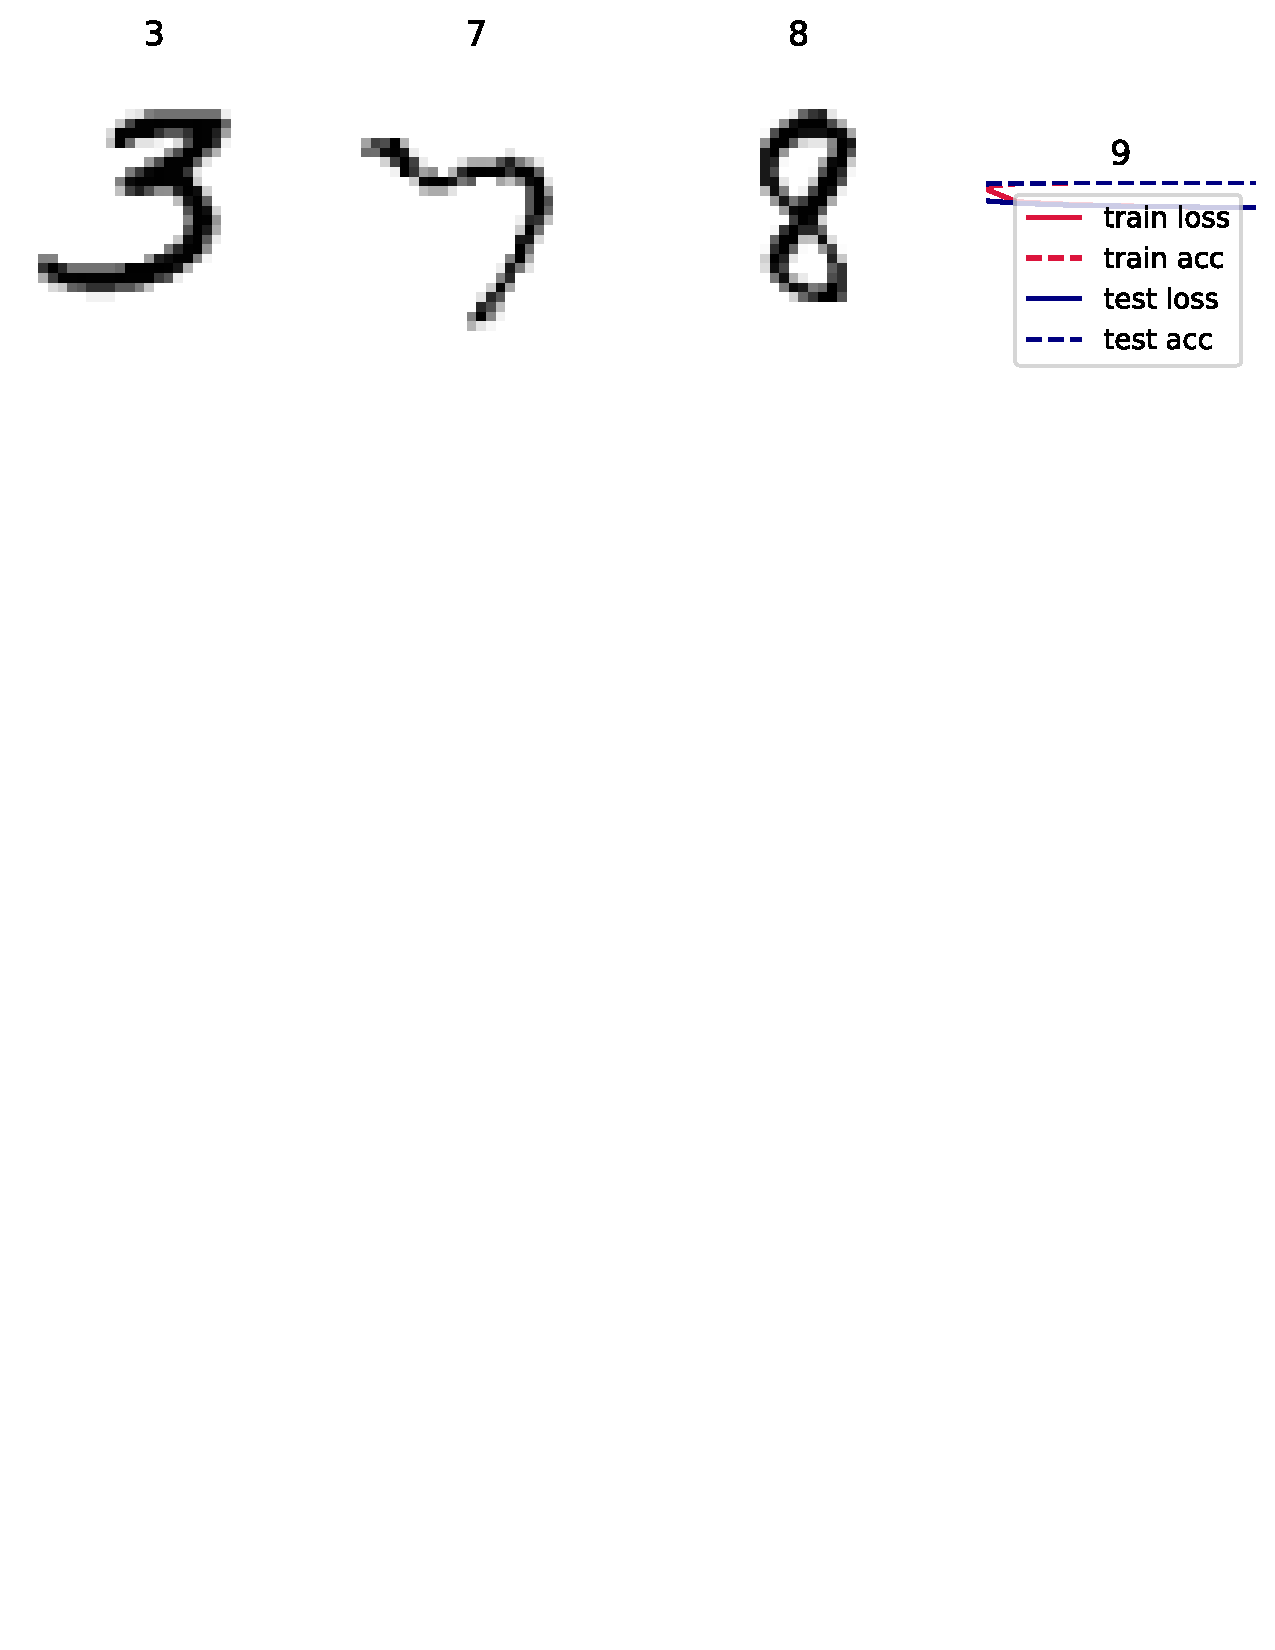
\includegraphics[width=0.6\textwidth]{data/training_graph.pdf}
        \caption{Training and test loss/accuracy over epochs.}
        \label{fig:training}
      \end{figure}

      \vspace{0.5em}
      \textbf{Code:}
      \begin{lstlisting}[language=Python]
import torch
import torch.nn.functional as F

# Define network dimensions
n_inputs = 28 * 28     # Input dimension (28x28 images)
n_hiddens = 256        # Number of hidden units
n_outputs = 10         # Number of output classes

# Initialize weights and biases with gradient tracking enabled
W1 = torch.randn(n_inputs, n_hiddens, requires_grad=True)
b1 = torch.zeros(n_hiddens, requires_grad=True)
W2 = torch.randn(n_hiddens, n_outputs, requires_grad=True)
b2 = torch.zeros(n_outputs, requires_grad=True)

def relu(x):
    """
    Applies the ReLU activation elementwise.
    """
    return torch.clamp(x, min=0)

def softmax(X):
    """
    Applies the softmax function row-wise.
    """
    # Subtract the row-wise max for numerical stability
    exp_X = torch.exp(X - torch.max(X, dim=1, keepdim=True)[0])
    return exp_X / torch.sum(exp_X, dim=1, keepdim=True)

def net(X):
    """
    Forward pass of the neural network.
    
    :param X: A batch of images of shape (batch_size, 1, 28, 28)
    :return: A tensor of shape (batch_size, 10) where each row is a probability vector.
    """
    # Flatten the images
    X = X.reshape(-1, n_inputs)
    
    # First linear transformation and ReLU non-linearity
    H = X @ W1 + b1
    H = relu(H)
    
    # Second linear transformation and softmax non-linearity
    O = H @ W2 + b2
    O = softmax(O)
    
    return O

def cross_entropy(y_hat, y):
    """
    Computes the cross entropy loss.
    
    :param y_hat: Tensor of shape (batch_size, 10) with predicted probabilities.
    :param y: Tensor of shape (batch_size,) with true labels.
    :return: A tensor of shape (batch_size,) with the loss for each instance.
    """
    batch_size = y.shape[0]
    # Select the probabilities corresponding to the true labels
    probs = y_hat[range(batch_size), y]
    return -torch.log(probs)

def sgd(params, lr=0.1):
    """
    Performs a stochastic gradient descent update.
    
    :param params: A list of parameters to update.
    :param lr: The learning rate.
    """
    with torch.no_grad():
        for param in params:
            if param.grad is not None:
                param -= lr * param.grad
                param.grad.zero_()

def train(net, params, train_iter, loss_func=cross_entropy, updater=sgd):
    """
    Trains the network for one epoch.
    
    :param net: The neural network function.
    :param params: The parameters of the network.
    :param train_iter: An iterator over the training data.
    :param loss_func: The loss function.
    :param updater: The optimizer function.
    """
    for X, y in train_iter:
        y_hat = net(X)
        loss = loss_func(y_hat, y).mean()
        loss.backward()
        updater(params, lr=0.1)
      \end{lstlisting}

    \item[2.]
      \textbf{Discussion of Training Trends:} \\
      In the training process, both the training and test loss decrease over epochs while the corresponding accuracies increase. This indicates that the network is learning the digit representations effectively. The smooth convergence and high final accuracies suggest that the model generalizes well on in-distribution data. Minor fluctuations observed during training are typical due to mini-batch variability.

    \item[3.]
      \textbf{Out-of-Distribution (OOD) Analysis:} \\
      \textbf{Test Accuracy (In Distribution):} 0.9955 \\
      \textbf{Test Accuracy (Out of Distribution):} 0.0 \\[0.5em]
      \textbf{Discussion:} \\
      The model attains near-perfect accuracy on in-distribution test data, confirming its strong performance on familiar images. However, its failure (0\% accuracy) the network is unable to correctly classify inputs that differ significantly from the training distribution. This sharp drop in performance underscores the need for more robust uncertainty estimation methods, which might flag such unfamiliar inputs for human review or additional processing.

    \item[4.]
      \textbf{Analysis of Predictive Uncertainties:} \\
       for in-distribution images, the model sometimes outputs a nearly uniform probability distribution when the digit is ambiguous or poorly drawn—indicating uncertainty. For OOD examples, the output probabilities are almost uniform across all classes, reflecting maximal uncertainty. While these uncertainty measures help identify potentially problematic inputs, they are not entirely reliable for automated decision-making. Integrating multiple models via bootstrapping could average out overconfident predictions and yield a more robust uncertainty estimate.

    \item[5.]
      \textbf{Safeguards against Adversarial Attacks:} \\
      \begin{enumerate}
        \item \textbf{Hardware Attack:} Protect the scanner by implementing tamper-proof hardware 
        \item \textbf{Input Attack:}  pre-processing, adversarial Training
        \item \textbf{Social Engineering Attack:} strict access control policies
      \end{enumerate}
  \end{enumerate}

\end{answer}



%%%%%%%%%%%%%%%%%%%%%%%%%%%%%%%%%%%%%%%%%%%%%
% Name and Calibration
%%%%%%%%%%%%%%%%%%%%%%%%%%%%%%%%%%%%%%%%%%%%%
\newpage
\subsection*{Matt Krasnow}

\subsection*{Nah}
CHATGPT for formatting LaTex from my handwritten notes

\end{document}
